\pdfinfoomitdate=1
\pdftrailerid{}
\pdfsuppressptexinfo=15
\documentclass[11pt]{article}
\usepackage[T1]{fontenc}
\usepackage{lmodern,microtype}
\usepackage[margin=1.08in]{geometry}
\usepackage{amsmath,amssymb,amsthm,mathtools}
\usepackage{tikz-cd}
\usepackage{booktabs}
\usepackage[colorlinks=true,linkcolor=blue!45!black,citecolor=blue!45!black,urlcolor=blue!45!black]{hyperref}
\hypersetup{pdftitle={A Complete Local Domain without a Small Cohen--Macaulay Module},pdfauthor={OpenAI}}
\newtheorem{theorem}{Theorem}[section]
\newtheorem{proposition}[theorem]{Proposition}
\newtheorem{lemma}[theorem]{Lemma}
\newtheorem{corollary}[theorem]{Corollary}
\theoremstyle{remark}
\newtheorem{remark}[theorem]{Remark}
\newcommand{\C}{\mathbb C}
\newcommand{\PP}{\mathbb P}
\newcommand{\cO}{\mathcal O}
\newcommand{\cE}{\mathcal E}
\newcommand{\cI}{\mathcal I}
\newcommand{\cJ}{\mathcal J}
\DeclareMathOperator{\Spec}{Spec}
\DeclareMathOperator{\rk}{rk}
\DeclareMathOperator{\ch}{ch}
\DeclareMathOperator{\Tor}{Tor}
\DeclareMathOperator{\depth}{depth}
\DeclareMathOperator{\Frac}{Frac}
\DeclareMathOperator{\Tot}{Tot}
\title{A Complete Local Domain without\\a Small Cohen--Macaulay Module}
\author{OpenAI}
\date{September 23, 2026}
\begin{document}
\maketitle
\begin{abstract}
We construct a three-dimensional complete Noetherian normal local domain
containing $\C$, with residue field $\C$, that has no nonzero finitely generated
maximal Cohen--Macaulay module. This disproves the domain form of the small
Cohen--Macaulay module conjecture.
\end{abstract}
\tableofcontents
\clearpage

\section{Introduction}
A \emph{small Cohen--Macaulay module} over a Noetherian local ring $(R,\mathfrak m)$
is a nonzero finitely generated $R$-module $M$ such that
$\depth_R M=\dim R$. Such a module is also called a maximal Cohen--Macaulay
module. The domain form of the small Cohen--Macaulay module conjecture asks
whether every complete Noetherian local domain has one.
We prove the following negative answer.

\begin{theorem}\label{thm:main}
There exists a three-dimensional complete Noetherian normal local domain
$R$ containing $\C$, with residue field $\C$, such that no nonzero finitely
generated $R$-module has depth three.
\end{theorem}

The distinction between modules and algebras matters here. A module-finite extension domain $R\subseteq B$ that is
Cohen--Macaulay supplies such a module, but the converse need not hold. Our obstruction applies to every finite module;
it requires neither a grading nor an algebra structure.
Hochster formulated the finite-module existence problem in his early
work on Cohen--Macaulay modules and homological conjectures
\cite{Hochster1973,Hochster1975}. In dimensions at most two, a complete
local domain has a small Cohen--Macaulay module: its finite normalization
is Cohen--Macaulay \cite[Section~2]{Hochster2017}. There are also important
positive results in the graded setting. The theorem of Hartshorne,
Peskine--Szpiro, and Hochster gives graded small Cohen--Macaulay modules
for three-dimensional finitely generated nonnegatively graded domains
whose degree-zero part is a perfect field of positive characteristic; see
\cite[Theorem~5.2]{HochsterYao2023} for the statement and historical
attribution. These results do not cover the characteristic-zero cones
considered here. Hochster's later account explicitly records both his
early existence conjecture and his subsequent expectation of counterexamples
\cite[Section~2, Conjectures~2.1 and 2.2]{Hochster2017}.

Dropping finite generation changes the problem. In the balanced convention,
a \emph{big Cohen--Macaulay module} is a possibly infinitely generated
module on which every system of parameters is a regular sequence and whose
quotient by the maximal ideal is nonzero. Hochster proved existence in
equal characteristic \cite{Hochster1975}. Hochster--Huneke showed that
the absolute integral closure of an excellent local domain of positive
characteristic is such an algebra \cite{HochsterHuneke1992}. Perfectoid
methods later yielded big Cohen--Macaulay algebras in mixed characteristic,
completing the existence theorem for Noetherian local rings
\cite[Theorem~0.7.1]{Andre2018}. These results impose no finite-generation
conclusion.

For a normal local domain containing the rational numbers, trace makes
the ring a direct summand of every module-finite extension domain. A
Cohen--Macaulay extension would therefore force the original ring to be
Cohen--Macaulay. Bhatt constructed positive-characteristic complete normal
local domains with no finite Cohen--Macaulay extension, using a Witt-vector
cohomological obstruction \cite{Bhatt2014}. Neither obstruction excludes
arbitrary finite modules. Bhatt, Hochster, and Ma instead study asymptotic
substitutes for small Cohen--Macaulay modules. Their August~25, 2026 version
describes the existence problem as open even for local rings at maximal
ideals of affine three-dimensional domains over algebraically closed
fields \cite[Sections~1.1 and 1.3]{BhattHochsterMa}.

The geometric input is a smooth integral projective surface $X$ over $\C$
with an ample
globally generated line bundle $\cO_X(H)$. Write
\[
 T(X,H)=\bigoplus_{j\geq0}H^0(X,\cO_X(jH)),\qquad
 R(X,H)=\widehat{T(X,H)_{T(X,H)_{>0}}}.
\]
Here the hat denotes completion at the maximal ideal. We write $K_X$ for
the canonical divisor and $c_2(X)$ for the second Chern number.
For the specific pair $(X,H)$ used for Theorem~\ref{thm:main}, the
uncompleted vertex localization $T(X,H)_{T(X,H)_{>0}}$ also has no small
Cohen--Macaulay module (Corollary~\ref{cor:affine-local}). It is a
three-dimensional local domain essentially of finite type over $\C$, so
this supplies a counterexample in the affine-local class just described.
The deduction uses faithful flatness of completion.
Our main intermediate result is the following obstruction.

\begin{theorem}\label{thm:obstruction}
Let $X$ be a smooth integral projective surface over $\C$, and let $H$ be
an ample globally generated divisor. If $R(X,H)$ admits a small
Cohen--Macaulay module, then
\begin{equation}\label{eq:obstruction}
 K_X^2-2c_2(X)\leq 6H^2.
\end{equation}
\end{theorem}

A numerical obstruction for Ulrich sheaves on surfaces follows from
Bogomolov's inequality and the Hodge index theorem. Beauville presented
this route for surfaces of N\'eron--Severi rank one
\cite[pp.~18--20]{Beauville2017}; Anghel gives the surface inequality
without that N\'eron--Severi rank restriction
\cite[Proposition~2.1 and Remark~2.3]{Anghel2026}.
For a projective surface, an Ulrich sheaf has trivial vector-bundle
pushforward under a finite linear projection to $\PP^2$
\cite[Proposition 2.1]{EisenbudSchreyer2003}. The argument
here replaces that triviality condition by a comparison of coherent
extensions across the exceptional divisor of a completed cone.
A module over the completed local ring need not carry a grading.
We therefore retain its actual vector bundle on the punctured spectrum,
rather than assume it descends to an Ulrich sheaf on $X$.
It is this comparison that permits arbitrary nongraded modules.
The explicit surface used below is the complete-quadrangle
Hirzebruch--Kummer construction appearing in \cite[Section 7.2]{Anghel2026}.
We give its construction and all the required numerical and positivity
checks directly.

There are two further recent comparisons. Anghel's September~14, 2026
preprint excludes arithmetically Cohen--Macaulay bundles under the
sharper inequality $K_X^2-2c_2(X)>3H^2$, and excludes graded maximal
Cohen--Macaulay modules over the same complete-quadrangle section rings
used here \cite[Theorems~1.1 and 1.3, Corollary~4.3]{Anghel2026Graded}.
That statement does not assert nonexistence of arbitrary modules over
the vertex completion. Chen's September~21, 2026 preprint proposes a
quantitative local-cohomology bound for every nonzero finite reflexive
module over a completed cone when $K_X\equiv4H$ and
$15H^2/8-\chi(\cO_X)>0$, and obtains a proposed completed-local
counterexample from the exponent-six cover
\cite[Main claim~1.1 and Consequence~1.2]{Chen2026}.
Thus the existential completed-module claim overlaps with that work.
Our obstruction applies without the proportionality hypothesis on
$K_X$ and $H$; the exponent-seven polarization used below has
$K_X\equiv5H$.\footnote{The two Anghel preprints disclose ChatGPT and
Claude assistance for exploratory computations, literature search and
editorial work. Chen discloses ChatGPT/OpenAI assistance in mathematical
development, checking, computations, literature and writing.}

\subsection*{Proof overview}
Choose a finite morphism $f:X\to\PP^2$ with
$f^*\cO_{\PP^2}(1)=\cO_X(H)$, and put $h=H^2=\deg f$.
The completed cone is finite over the regular local ring
$A=\C[[x_0,x_1,x_2]]$. A small Cohen--Macaulay module is free over $A$.
Its restriction to the punctured cone is a vector bundle, which extends
to a coherent sheaf $\cE$ on a regular model $W\to\Spec R(X,H)$
that is an isomorphism away from the exceptional surface $X$.

For a nonzero torsion-free sheaf $B$ on $X$, its normalized slope is
\[
 \mu(B)=\frac{c_1(B)\cdot H}{\rk(B)H^2}.
\]
It is slope-semistable if no nonzero subsheaf of smaller rank has larger
slope. Its Harder--Narasimhan filtration has torsion-free semistable
factors with decreasing slopes.
We choose $\cE$ with torsion-free restriction $P=\cE|_X$.
First, elementary modifications of $\cE$ along $X$ arrange that the
slopes of the Harder--Narasimhan factors of $P$ lie in an interval of
length at most one. These modifications preserve the bundle away from
$X$. Second, that bundle comes from an $A$-free module. Comparing the
pushforward of $\cE$ with a trivial sheaf on the blowup of $\Spec A$
gives, for $F=f_*P$ of rank $N$, the inequality
$2N\ch_2(F)\geq c_1(F)^2$, with Chern characters evaluated on $\PP^2$.
Bogomolov's inequality for the semistable factors bounds the same
normalized Chern expression above. More precisely, if $r=\rk P$,
then $N=rh$ and the two comparisons give
\[
 0\leq \frac{2\ch_2(f_*P)}{N}
        -\left(\frac{c_1(f_*P)}{N}\right)^2
 \leq\frac12-\frac{K_X^2-2c_2(X)}{12H^2}.
\]
This yields \eqref{eq:obstruction}. Neither $P$ nor $f_*P$ is
assumed semistable or Ulrich.

Section~\ref{sec:cone} constructs the resolution and extends an arbitrary
module. Section~\ref{sec:balancing} proves the slope modification lemma.
Section~\ref{sec:lattice} establishes the Chern-character inequality,
and Section~\ref{sec:numerical} combines it with surface theory.
Finally, Section~\ref{sec:surface} constructs a surface with
$K_X^2-2c_2(X)>6H^2$.

\section{From a completed cone to its exceptional surface}\label{sec:cone}
Throughout this section, $X$ and $H$ satisfy the hypotheses of
Theorem~\ref{thm:obstruction}. We construct a regular model of the
completed cone and explain how a small Cohen--Macaulay module produces a
sheaf on it. We also prove that the completed ring is normal.

\subsection{The finite map and the completed ring}
Global generation supplies sections $s_0,s_1,s_2$ of $\cO_X(H)$ with no
common zero. Indeed, choose $s_0\ne0$, then $s_1$ avoiding the components
of its zero divisor, and then $s_2$ nonvanishing at their finitely many
common zeros. The resulting morphism
\[
 f:X\longrightarrow D:=\PP^2,\qquad f^*\cO_D(1)=\cO_X(H),
\]
is finite and surjective. A positive-dimensional fiber would contain a
curve on which $H$ is both ample and trivial, which is impossible.
Properness then gives finiteness, and the intersection formula gives
$\deg f=h:=H^2$.

Put
\[
 S=\C[x_0,x_1,x_2],\quad T=T(X,H),\quad
 A=\C[[x_0,x_1,x_2]],\quad R=T\otimes_S A,
\]
where $x_i$ acts as $s_i$. Surjectivity of $f$ makes $S\to T$ injective.
The ring $T$ is a domain, as seen by trivializing $H$ rationally and
embedding $T$ in $\C(X)[t]$. It is a finite graded $S$-module: by the
projection formula, its graded pieces are the nonnegative twisted
sections of the coherent sheaf $f_*\cO_X$ on $D$, and Serre vanishing
implies finite generation. Explicitly, a surjection
$\cO_D(-a)^p\to f_*\cO_X$ and the vanishing of the first cohomology of its
kernel in large twists generate all sufficiently large degrees;
the remaining finitely many degrees complete a generating set.

Let $\mathfrak n=T_{>0}$ and $\mathfrak a=(x_0,x_1,x_2)T$.
The $\mathfrak a$-adic filtration is cofinal with the degree filtration:
if homogeneous $S$-module generators have degrees at most $a'$, then
\[
 \mathfrak a^j\subseteq T_{\geq j},\qquad
 T_{\geq j+a'}\subseteq\mathfrak a^j.
\]
Finiteness over $S$ and completion of finite modules
\cite[Tags~00MA and 00MB]{Stacks} therefore identify
\begin{equation}\label{eq:completion}
 R=\widehat T^{\,\mathfrak a}=\prod_{j\geq0}T_j
   =\widehat{T_{\mathfrak n}},
\end{equation}
with multiplication by the graded Cauchy product. The product of the
first nonzero homogeneous terms proves that $R$ is a domain. An element
with nonzero constant term is a unit. Moreover, $T/\mathfrak a$ is a
finite-dimensional positively graded algebra with degree-zero part
$\C$, so $\sqrt{\mathfrak a}=\mathfrak n$. This justifies the last equality
in \eqref{eq:completion} and shows that $R$ is a complete Noetherian
local ring with residue field $\C$. Flatness of $S\to A$ gives an
injection $A\to R$; this finite integral extension has dimension three.

\subsection{The regular model and normality}
Let $V_0=\Tot(\cO_D(-1))$, the blowup of $\Spec S$ at the origin, and
let
\[
 W_0=X\times_D V_0=\Tot(\cO_X(-H)).
\]
The map $W_0\to V_0$ is finite. Evaluation of homogeneous sections gives
$W_0\to\Spec T$. It is an isomorphism off the zero section. To see this
without any assumption that $T$ is generated in degree one, set
$X_i=\{s_i\ne0\}$. The set $X_i$ is affine, and clearing poles along
the zero divisor of $s_i$ gives
\[
 T[1/s_i]=\Gamma(X_i,\cO_{X_i})[s_i,s_i^{-1}].
\]
Both the punctured line bundle over $X_i$ and the corresponding open
subset of $\Spec T$ have this coordinate ring.

Base change along $S\to A$ to obtain $g:W\to V$ and
$p:W\to\Spec R$. The zero sections remain $X\subset W$ and $D\subset V$.
Their ideal sheaves $\cJ$ and $\cI$ satisfy
\begin{equation}\label{eq:conormal}
 \cJ=g^*\cI,\qquad \cI|_D=\cO_D(1),\qquad
 \cJ|_X=\cO_X(H).
\end{equation}
The zero sections are Cartier divisors by flatness. The relevant maps
fit into the diagram
\[
\begin{tikzcd}[column sep=large,row sep=large]
 X \arrow[r,hook] \arrow[d,"f"'] & W \arrow[r,"p"] \arrow[d,"g"]
 & \Spec R \arrow[d] \\
 D \arrow[r,hook] & V \arrow[r] & \Spec A .
\end{tikzcd}
\]
The maps $g$ and $\Spec R\to\Spec A$ are finite, and $V$ and $W$ are
proper over $\Spec A$. Since $\Spec R$ is separated over $\Spec A$,
the map $p$ is proper as well. The maps $p$ and $V\to\Spec A$ identify
$W\setminus X$ and $V\setminus D$ with the punctured spectra of $R$
and $A$, respectively.

Both $V$ and $W$ are regular. At a point of the closed fiber, a local
Cartier equation is a nonzerodivisor and its quotient local ring is
regular, since $D$ and $X$ are smooth. Lifting generators of the quotient
maximal ideal shows that the embedding dimension is at most one more
than the quotient dimension; the nonzerodivisor raises dimension by
one. The local ring is therefore regular. Properness over the local
base ensures that the closure of every point meets the closed fiber.
Regularity at all other points follows by localization. A regular
Noetherian scheme has disjoint irreducible components; here every
component meets the integral closed fiber, so each of $V$ and $W$ is
integral.

This model also proves normality of $R$. The line bundle projection
$W_0\to X$ identifies its global functions with $T$.
Flat base change \cite[Tag 02KH]{Stacks} then gives
\begin{equation}\label{eq:global-sections}
 \Gamma(W,\cO_W)=\Gamma(W_0,\cO_{W_0})\otimes_S A=R.
\end{equation}
For this equality, take a finite affine cover of the separated scheme
$W_0$ and tensor the kernel computing global sections with the flat
$S$-algebra $A$. The global functions on an integral normal scheme form
an integrally closed domain: a fraction integral over the global ring
is integral over every local ring, hence regular everywhere.
Since $W$ is regular and integral, \eqref{eq:global-sections} proves
that $R$ is normal.

\subsection{Extending an arbitrary module}
Suppose that $M$ is a small Cohen--Macaulay $R$-module. The parameters
$x_0,x_1,x_2$ form an $M$-regular sequence, so $M$ has depth three over
$A$. The Auslander--Buchsbaum formula over the regular local ring $A$
\cite[Tags~00N6, 00O7 and 090V]{Stacks}
shows that
\begin{equation}\label{eq:A-free}
 M\simeq A^N\quad\text{as an $A$-module},\qquad N>0.
\end{equation}
The localization $R\otimes_A\Frac(A)$ is a finite-dimensional domain
over a field, hence a field. Thus $M$ has positive generic rank over
$R$ and full support.

The restriction of $M$ to the punctured spectrum is locally free.
Indeed, Cohen--Macaulay modules of full support localize to
Cohen--Macaulay modules. More explicitly, for a prime $\mathfrak q$ the
depth localization inequality \cite[Tag 0FCC]{Stacks} gives
\[
 \depth_{R_{\mathfrak q}}M_{\mathfrak q}
 \geq 3-\dim(R/\mathfrak q)\geq\dim R_{\mathfrak q}.
\]
The second inequality follows by concatenating chains of primes below
and above $\mathfrak q$. On the puncture $R_{\mathfrak q}$ is regular
by the model $W$, and Auslander--Buchsbaum gives freeness.

On $W$, take
\[
 \cE=(p^*\widetilde M)^{**},\qquad P=\cE|_X,
\]
where duals are over $\cO_W$. Then $\cE$ is coherent and torsion-free,
and agrees with $M$ away from $X$. The restriction $P$ is torsion-free
of positive rank on $X$. Here is the local justification. On a regular integral
scheme a coherent dual has depth at least $\min(2,\dim\cO_{W,w})$:
dualizing a finite presentation expresses it as a kernel of a map
between finite free modules, whose image is torsion-free, and the depth
lemma applies. At any nongeneric point of $X$, quotienting $\cE$ by the
Cartier equation therefore leaves depth at least one. Thus $P$ has no
associated points except the generic point of $X$. At that generic
point $\cE$ is free over a discrete valuation ring, so $P$ has the same
positive rank as $\cE$.

Finally, $g_*\cE$ is torsion-free and, by \eqref{eq:A-free}, agrees with
$\cO_V^N$ off $D$. We have obtained the precise input for the next two
sections: a sheaf that can be modified along $X$, whose pushforward
remains trivial away from $D$.

\section{Balancing slopes by modifications}\label{sec:balancing}
We now modify the extension along $X$ so that its restriction has
Harder--Narasimhan slopes in an interval of length at most one.
Recall the normalization $\mu(B)=c_1(B)\cdot H/(\rk(B)h)$, where
$h=H^2$. Tensoring with $\cO_X(H)$ increases slope by one.

Elementary modification to constrain the slopes of exceptional-divisor
restrictions has an antecedent in Chen--Sun's optimal extensions of
reflexive analytic sheaves \cite[Theorem~1.4(I), Proposition~2.6 and
Remark~1.5]{ChenSun2020}. Their analytic setting and reflexivity
hypotheses differ from the Noetherian Cartier-divisor setting below;
we give the needed algebraic modification and termination argument.

We recall briefly why the filtration exists in this setting.
A torsion-free sheaf embeds in a sum of sufficiently positive line
bundles, so its subsheaf slopes are bounded above by taking determinants.
Their denominators are bounded because their ranks are bounded.
Choose a subsheaf of maximum slope and, among these, of maximum rank;
saturate it. Saturation does not decrease degree, since a torsion
sheaf has effective divisorial first Chern class. The chosen subsheaf
is semistable, and every subsheaf of its torsion-free quotient has
strictly smaller slope. Induction on rank gives the filtration.
This is the usual construction of the Harder--Narasimhan filtration
\cite[Section~1.6, Theorem~1.6.7 and Definition/Corollary~1.6.9]{HuybrechtsLehn}.

\begin{lemma}\label{lem:balance}
Let $W$ be an integral Noetherian scheme, let $i:X\hookrightarrow W$ be
an effective Cartier divisor that is a smooth integral projective surface
over $\C$, and
suppose its ideal $\cJ$ restricts to an ample line bundle $\cO_X(H)$.
Let $\cE$ be a coherent torsion-free sheaf on $W$ such that
$P=\cE|_X$ is torsion-free of positive rank.
There is a coherent torsion-free sheaf $\cE'$ agreeing with $\cE$ off
$X$ such that $P'=\cE'|_X$ is torsion-free and the normalized slopes of
its Harder--Narasimhan factors lie in an interval of length at most one.
\end{lemma}
\begin{proof}
Suppose the current largest and smallest factor slopes differ by more
than one. Let $G$ be the last semistable quotient of $P$, and let
$B=\ker(P\to G)$. Replace $\cE$ by
$\cE'=\ker(\cE\to i_*G)$. This is torsion-free and unchanged off $X$.
The Cartier resolution gives
\begin{equation}\label{eq:transform}
 0\longrightarrow G(H)\longrightarrow \cE'|_X
   \longrightarrow B\longrightarrow0.
\end{equation}
Indeed, $\Tor_1^W(\cE,\cO_X)=0$ because the Cartier equation acts
injectively on $\cE$, whereas
\[
 \Tor_1^W(i_*G,\cO_X)=G\otimes\cJ|_X=G(H).
\]
Thus the new restriction remains torsion-free of the same rank $r$.

The maximum slope of an extension of torsion-free sheaves is at most
the larger of their maximum slopes: intersect a subsheaf with the
kernel and take its image in the quotient. Since
$\mu(G)+1<\mu_{\max}(P)$, \eqref{eq:transform} shows that the maximum
slope does not increase. On the other hand, additivity of rank and
first Chern class gives
\[
 \mu(\cE'|_X)=\mu(P)+\frac{\rk G}{r}\geq\mu(P)+\frac1r.
\]
The average slope is always bounded above by the maximum slope, hence
by the initial maximum. Consequently this procedure terminates after
finitely many steps. At termination the slope interval has length at
most one.
\end{proof}

Apply Lemma~\ref{lem:balance} to the sheaf constructed in
Section~\ref{sec:cone}, and again call the resulting sheaves $\cE$ and
$P$. The rank and the bundle on the puncture are unchanged.
In particular, $g_*\cE$ still agrees with $\cO_V^N$ off $D$.
The restriction $P$ need not be semistable: it is the width of its
factor slopes, rather than semistability, that we have arranged.
This agreement on the puncture imposes the lower bound proved next.

\section{A Chern-character inequality from a divisor}\label{sec:lattice}
The pushforward of our extension agrees with a trivial bundle away
from $D$. We show that this agreement forces a nonnegative expression
in the Chern characters of its restriction to $D$.
For a coherent sheaf $F$ of positive rank $N$ on $D=\PP^2$, identify
$c_1(F)$ with its integer coefficient in the line class, and let
$\ch_2(F)$ mean the degree of the second Chern character. Define
\[
 v(F)=\frac{2\ch_2(F)}N-\left(\frac{c_1(F)}N\right)^2.
\]
For $F=\bigoplus_{i=1}^N\cO_D(a_i)$, this is the ordinary variance
of the integers $a_i$. It need not be nonnegative for arbitrary sheaves.
The expression is unchanged by twisting $F$ by $\cO_D(b)$.

\begin{lemma}\label{lem:lattice}
Let $V$ be an integral Noetherian scheme with an effective Cartier
divisor $D\simeq\PP^2$, whose ideal $\cI$ satisfies
$\cI|_D\simeq\cO_D(1)$. Suppose $L'$ is a coherent torsion-free sheaf
on $V$ and $L'|_{V\setminus D}\simeq\cO_{V\setminus D}^N$, where $N>0$.
Then $F=L'|_D$ has rank $N$ and $v(F)\geq0$.
\end{lemma}
\begin{proof}
At the generic point of $D$, the local ring of $V$ has maximal ideal
generated by the Cartier equation, so it is a discrete valuation ring.
The torsion-free sheaf $L'$ is free of rank $N$ there; hence $F$ has rank
$N$ and $v(F)$ is defined.
Write $L=\cO_V^N$ and identify $L$ and $L'$ after inverting the Cartier
equation. Clearing denominators on a finite affine cover gives
\[
 \cI^b L\subseteq L'\subseteq\cI^{-b}L
\]
for some $b\geq0$. Replacing $L'$ by $L'\otimes\cI^b$ replaces $F$ by
$F(b)$ and does not change $v(F)$. We may therefore assume
$\cI^{2b}L\subseteq L'\subseteq L$.

The quotient $Q=L/L'$ is killed by a power of $\cI$. Its finite
filtration has factors
\[
 Q_j=\cI^jQ/\cI^{j+1}Q\qquad(j\geq0)
\]
on $D$. Each $Q_j$ is a quotient of $\cO_D(j)^N$. If $n_j=\rk Q_j$,
then
\begin{equation}\label{eq:layers}
 0\leq n_j\leq N,\qquad c_1(Q_j)\geq jn_j.
\end{equation}
For the second assertion, $Q_j(-j)$ is globally generated. The
determinant of its torsion-free quotient has a nonzero section, and its
torsion contributes a nonnegative divisorial first Chern class.

Derived restriction to $D$ gives the following identity in the
Grothendieck group of coherent sheaves on $D$:
\begin{equation}\label{eq:Tor}
 [F]=[\cO_D^N]+\sum_{j\geq0}\bigl([Q_j(1)]-[Q_j]\bigr).
\end{equation}
Indeed, restriction minus first Tor is additive, with no higher Tor
against a Cartier divisor. The first Tor vanishes for $L,L'$, while
for a sheaf $Q_j$ supported on $D$ it equals $Q_j(1)$.
Taking Chern characters in \eqref{eq:Tor} gives rank $N$ and
\[
 c_1(F)=\sum_j n_j,\qquad
 2\ch_2(F)=\sum_j\bigl(2c_1(Q_j)+n_j\bigr)
 \geq\sum_j(2j+1)n_j.
\]
The remaining assertion is the elementary inequality
\begin{align*}
 N\sum_j(2j+1)n_j-\left(\sum_jn_j\right)^2
 &=\sum_jn_j(N-n_j)
   +2\sum_{j>\ell}n_j(N-n_\ell)\geq0,
\end{align*}
which follows from \eqref{eq:layers}. Dividing by $N^2$ proves the lemma.
\end{proof}

For $L'=g_*\cE$, the equality $\cJ=g^*\cI$ in
\eqref{eq:conormal} and finite pushforward give
\[
 L'|_D=f_*P.
\]
Writing $r=\rk P$, this sheaf has rank $rh$ by finite pushforward
along $f$, and rank $N$ by generic restriction along $D$ in
Lemma~\ref{lem:lattice}. Thus the two ranks agree: $N=rh$.
The hypotheses of Lemma~\ref{lem:lattice} hold by
\eqref{eq:conormal} and the construction of $\cE$.
Consequently
\begin{equation}\label{eq:lower}
 v(f_*P)\geq0.
\end{equation}
It remains to bound this expression above using the narrow slope
interval of $P$.

\section{The numerical obstruction}\label{sec:numerical}
We first compute the contribution of one semistable factor.
We use surface Riemann--Roch and the Hodge index theorem in their
standard forms; see \cite[Appendix A, Theorem 4.1 and Example 4.1.2;
Chapter V, Theorem 1.9]{Hartshorne}.
On each smooth projective surface, finite locally free resolutions
extend Riemann--Roch additively to coherent sheaves
\cite[Appendix~A, Section~5]{Hartshorne}. This covers the possibly
non-locally-free sheaves $G$ and $f_*G$ below; we compare their Euler
characteristics, without requiring the finite morphism $f$ to be smooth.
All intersections in this section are on $X$, except for Chern
characters explicitly taken on $D=\PP^2$.

\begin{lemma}\label{lem:factor}
Let $f:X\to\PP^2$ be finite, with $X$ a smooth integral projective
complex surface and $H=f^*\cO_{\PP^2}(1)$ ample. Put $h=H^2$.
For every nonzero torsion-free $H$-slope-semistable sheaf $G$ on $X$,
\[
 v(f_*G)\leq\frac14-\frac{K_X^2-2c_2(X)}{12h}.
\]
Moreover,
$\displaystyle\frac{c_1(f_*G)}{\rk(f_*G)}
=\mu(G)-\frac{K_X\cdot H}{2h}-\frac32$.
\end{lemma}
\begin{proof}
Write $u=\rk G$, $k=K_X\cdot H$, and
\[
 m=\frac{c_1(f_*G)}{uh},\qquad q=\frac{\ch_2(f_*G)}{uh}.
\]
The rank of $f_*G$ is $uh$. Finite pushforward and the projection formula
identify the twist Euler characteristics on $X$ and $\PP^2$.
Surface Riemann--Roch, divided by $uh$, therefore gives
\begin{align*}
 \frac{t^2}{2}+\left(\frac32+m\right)t+1+\frac32m+q
 =\frac{t^2}{2}+\left(\mu(G)-\frac{k}{2h}\right)t
 +\frac{\chi(\cO_X)}h
 +\frac{\ch_2(G)}{uh}-\frac{c_1(G)\cdot K_X}{2uh}.
\end{align*}
Comparison of the linear coefficients proves the formula for $m$.
Comparison of constants, followed by completing the square, yields
\begin{equation}\label{eq:RR-variance}
 2q-m^2=\frac14+\frac{2\chi(\cO_X)}h
 +\frac{2\ch_2(G)/u-c_1(G)\cdot K_X/u}{h}
 -\left(\mu(G)-\frac{k}{2h}\right)^2.
\end{equation}

Bogomolov's inequality for a torsion-free slope-semistable sheaf on a
smooth projective complex surface states that
\[
 2u\ch_2(G)\leq c_1(G)^2
\]
\cite[Theorem 3.4.1]{HuybrechtsLehn}. Its hypotheses apply to $G$ and the ample
polarization $H$; normalizing slope by $h$ does not change semistability.
Set $C=c_1(G)/u-K_X/2$. The last two terms of
\eqref{eq:RR-variance} are at most
\[
 \frac{C^2-K_X^2/4}{h}-\frac{(C\cdot H)^2}{h^2}
 \leq-\frac{K_X^2}{4h},
\]
by the Hodge index theorem for the rational divisor class $C$.
Using Noether's formula $12\chi(\cO_X)=K_X^2+c_2(X)$ now gives the result.
\end{proof}

\begin{proof}[Proof of Theorem~\ref{thm:obstruction}]
Starting with a small Cohen--Macaulay module, Sections~\ref{sec:cone}
and~\ref{sec:balancing} construct a torsion-free sheaf $P$ on $X$ whose
semistable factors $G_i$ have normalized slopes in an interval of length
at most one. Write $u_i=\rk G_i$, $r=\rk P$, and $w_i=u_i/r$.
Thus $w_i>0$ and $\sum_iw_i=1$. Finite pushforward is exact, so
$F=f_*P$ has rank $rh=N$, and its normalized Chern characters are the
weighted averages of those of $f_*G_i$.
If $m_i=c_1(f_*G_i)/(u_ih)$ and $\overline m=\sum_iw_i m_i$, then
\begin{equation}\label{eq:mixture}
 v(F)=\sum_iw_i v(f_*G_i)+\sum_iw_i(m_i-\overline m)^2.
\end{equation}
Lemma~\ref{lem:factor} shows that the $m_i$ differ from $\mu(G_i)$ by a
common constant. They therefore lie in an interval of length at most
one. Their weighted variance is at most $1/4$: the mean minimizes the
mean square distance, and every point is within $1/2$ of the interval
midpoint. Combining \eqref{eq:lower}, \eqref{eq:mixture}, and
Lemma~\ref{lem:factor} gives
\[
 0\leq v(F)\leq\frac12-\frac{K_X^2-2c_2(X)}{12h}.
\]
This is precisely \eqref{eq:obstruction}.
\end{proof}

\section{An explicit surface and its polarization}
\label{sec:surface}

We construct a family of smooth projective surfaces from which we will
choose one violating the inequality established above.  The construction uses the six lines joining
four points of the plane, followed by a cover obtained by taking roots of
their ratios.  The same line arrangement provides the sections needed for
an ample globally generated divisor on the cover.  This choice of
arrangement and polarization is the complete-quadrangle construction
in \cite[Section 7.2]{Anghel2026}; all properties needed here are verified below.

\begin{proposition}\label{prop:surface}
For each prime $n\geq3$, there is a smooth integral projective complex
surface $X$ with an ample globally generated divisor $H$ such that
\[
 H^2=5n^3,\qquad K_X^2-2c_2(X)=n^3(n^2-10).
\]
\end{proposition}

We prove the proposition by constructing the cover, checking its local
coordinates, and then finding sections of the required polarization.
The covering construction goes back to Hirzebruch's work on line
arrangements \cite{Hirzebruch1983}.

\subsection{The branch divisor}

Choose four points $p_1,\ldots,p_4\in\mathbb P^2_{\mathbb C}$, no three
collinear, and let $B$ be their blowup.  Write $\ell$ for the pullback of
the line class and $e_1,\ldots,e_4$ for the exceptional curves.  Thus
\[
 \ell^2=1,\qquad \ell\cdot e_i=0,\qquad
 e_i\cdot e_j=-\delta_{ij},\qquad
 K_B=-3\ell+\sum_{i=1}^4 e_i.
\]
Number the six joining lines from $1$ to $6$, and choose defining linear
forms $l_1,\ldots,l_6$.  Denote the strict transform of line $a$ by $L_a$
and its total transform by $T_a$.  If its endpoints are $p_i,p_j$, then
\[
 T_a=L_a+e_i+e_j\sim\ell.
\]
Two joining lines are called \emph{opposite} if their endpoint pairs are
disjoint.  There are three opposite pairs.

Let
\[
 \Delta=\sum_{a=1}^6 L_a+\sum_{i=1}^4e_i.
\]
This reduced divisor has simple normal crossings.  Each exceptional curve
meets the three incident strict transforms in three distinct points.
Strict transforms of lines with a common endpoint are disjoint, whereas
each opposite pair meets transversely in one point away from the
exceptional curves.  The three latter points are distinct: an equality
between two would force two lines with a common endpoint to meet away
from that endpoint.  Consequently $\Delta$ has ten rational components,
each meeting the others in three points, and fifteen nodes in total.
Figure~\ref{fig:branch-incidence} records these incidences; in the
figure $L_{ij}$ denotes the strict transform of the line joining
$p_i$ and $p_j$.
Since each point belongs to three joining lines,
\begin{equation}\label{eq:branch-class}
 \Delta\sim6\ell-2\sum_{i=1}^4e_i=-2K_B,
 \qquad K_B^2=5.
\end{equation}

\begin{figure}[htbp]
\centering
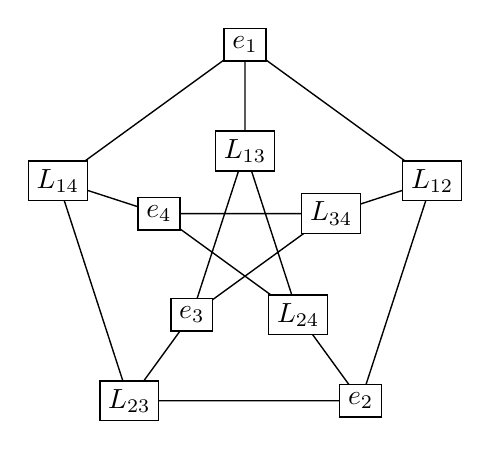
\begin{tikzpicture}[every node/.style={draw,fill=white,inner sep=3pt},
  line width=0.5pt]
\coordinate (outerone) at (90:2.5);
\coordinate (outertwo) at (18:2.5);
\coordinate (outerthree) at (-54:2.5);
\coordinate (outerfour) at (-126:2.5);
\coordinate (outerfive) at (162:2.5);
\coordinate (innerone) at (90:1.15);
\coordinate (innertwo) at (18:1.15);
\coordinate (innerthree) at (-54:1.15);
\coordinate (innerfour) at (-126:1.15);
\coordinate (innerfive) at (162:1.15);
\draw (outerone)--(outertwo)--(outerthree)--(outerfour)--(outerfive)--cycle;
\draw (outerone)--(innerone) (outertwo)--(innertwo)
      (outerthree)--(innerthree) (outerfour)--(innerfour)
      (outerfive)--(innerfive);
\draw (innerone)--(innerthree)--(innerfive)--(innertwo)--(innerfour)--cycle;
\node at (outerone) {$e_1$};
\node at (outertwo) {$L_{12}$};
\node at (outerthree) {$e_2$};
\node at (outerfour) {$L_{23}$};
\node at (outerfive) {$L_{14}$};
\node at (innerone) {$L_{13}$};
\node at (innertwo) {$L_{34}$};
\node at (innerthree) {$L_{24}$};
\node at (innerfour) {$e_3$};
\node at (innerfive) {$e_4$};
\end{tikzpicture}
\caption{The branch-incidence graph on the blown-up plane.
Vertices represent the ten rational components, not points of the
surface; edges represent its fifteen branch nodes. Twelve edges join
$e_i$ to an incident $L_{ij}$, and three join opposite line transforms.
Every vertex has degree three. Crossings of drawn graph edges do not
represent additional intersections.}
\label{fig:branch-incidence}
\end{figure}

\subsection{The cover and its local coordinates}

Fix a prime $n\geq3$, to be chosen at the end.  In an algebraic closure of
$K=\mathbb C(B)$ choose elements $y_a$ satisfying
\[
 y_a^n=l_a/l_6\qquad(1\leq a\leq5),
\]
and let $\pi:X\to B$ be the normalization of $B$ in
$K'=K(y_1,\ldots,y_5)$. The base $B$ is normal and Noetherian, and
this finite characteristic-zero field extension is separable.
Its normalization is therefore finite \cite[Tag~032L]{Stacks},
so $X$ is an integral projective surface.

\begin{lemma}\label{lem:cover-smooth}
The surface $X$ is smooth and $\deg\pi=d=n^5$.  The map is unramified
outside $\Delta$ and has ramification index $n$ along every component of
$\Delta$.  More precisely, near a point at which exactly $s\in\{0,1,2\}$
components of $\Delta$ meet, it is, after an \'{e}tale base change, the
disjoint union of $n^{5-s}$ copies of
\[
 (t_1,t_2)\longmapsto
 \begin{cases}
 (t_1,t_2),&s=0,\\
 (t_1^n,t_2),&s=1,\\
 (t_1^n,t_2^n),&s=2.
 \end{cases}
\]
Here the displayed maps are understood in \'{e}tale coordinates on the
base and the source.
\end{lemma}

\begin{proof}
First, suppose that integers $c_1,\ldots,c_5$ satisfy
\[
 \prod_{a=1}^5(l_a/l_6)^{c_a}\in K^{*n}.
\]
Taking valuations along $L_a$ shows that $n$ divides $c_a$ for every $a$.
Thus the five radicands are independent in $K^*/K^{*n}$.  Since $K$
contains the $n$th roots of unity, the extension $K'/K$ is Galois and its
group embeds in $(\mathbb Z/n)^5$ by its action on the roots.  If its
image were a proper subgroup, some nonzero linear functional on
$(\mathbb Z/n)^5$ would annihilate it.  The corresponding product of
the $y_a$ would then lie in $K$, contradicting the independence just
proved.  This gives $[K':K]=n^5$.

We next record the valuations modulo $n$ along the branch curves.  Use
the vector space
\[
 U_n=\mathbb F_n^6/\langle(1,1,1,1,1,1)\rangle
\]
and denote the images of its six standard vectors by
$\varepsilon_1,\ldots,\varepsilon_6$.  Identifying
$\varepsilon_1,\ldots,\varepsilon_5$ with the standard basis of
$\mathbb F_n^5$, the valuation vector along $L_a$ is
$\varepsilon_a$; in particular
$\varepsilon_6=-\sum_{a=1}^5\varepsilon_a$.  If $I_i$ is the set of
the three lines incident with $p_i$, the valuation vector along $e_i$ is
\[
 w_i=\sum_{a\in I_i}\varepsilon_a.
\]
All these vectors are nonzero.  At a node formed by two strict
transforms, the vectors are two distinct $\varepsilon_a$, hence are
independent.  At a node $L_a\cap e_i$, one has $a\in I_i$, and
$\varepsilon_a,w_i$ are independent as well.  Indeed, if
$\lambda\varepsilon_a+\mu w_i=0$ in $U_n$, a coordinate outside $I_i$
forces the corresponding constant vector to be zero.  A coordinate in
$I_i\setminus\{a\}$ then gives $\mu=0$, followed by $\lambda=0$.

It remains to check that this independence gives the asserted smooth
normalization, including at the nodes.  At a closed point of $B$, choose
regular parameters $u_1,u_2$ such that the local branches of $\Delta$
are $u_1=0,\ldots,u_s=0$.  Shrink to an affine neighborhood on which
these parameters define an \'{e}tale map to $\mathbb A^2$.  Each radicand
is a monomial in $u_1,\ldots,u_s$, with possibly negative exponents,
times a unit.  Adjoining $n$th roots of these units is an \'{e}tale base
change.  On an integral neighborhood of a point of that base change,
divide the $y_a$ by the resulting roots of the units.

The $s$ columns of exponents modulo $n$ are independent by the preceding
calculation.  Multiplicative changes of the five root generators by a
matrix in $\operatorname{GL}_5(\mathbb F_n)$ therefore reduce their
equations to
\[
 Y_j^n=u_j\quad(1\leq j\leq s),\qquad
 Y_j^n=1\quad(s<j\leq5).
\]
To make this reduction in the function field, lift the matrix entries
to integers and divide by suitable monomials in the $u_j$ to remove
exponents divisible by $n$.  The generator change is reversible because
its matrix is invertible modulo $n$.  It consequently describes the
whole generic algebra after base change, not merely a subextension.
The first $s$ equations generate a field of degree $n^s$, by the
valuations along $u_j=0$, and the remaining equations split completely.
The generic algebra is therefore a product of $n^{5-s}$ copies of that
field.

On this neighborhood, with coordinate ring $C$, the normalization in
each factor is
\[
 C[t_1,\ldots,t_s]/(t_1^n-u_1,\ldots,t_s^n-u_s),
\]
so the full normalization is a product of $n^{5-s}$ such algebras.
Indeed, this algebra is finite and free over $C$, has the indicated
generic field, and is smooth: it is the base change of the \'{e}tale
coordinate map to $\mathbb A^2$ along the corresponding coordinate
power map.  In particular it is normal, so it is the integral closure
of $C$ in that field.  Normalization commutes with this \'{e}tale base
change: the pullback of $X$ is normal and has the same generic algebra,
and is pure of dimension two, since it is \'{e}tale over the normal
integral surface $X$. Each component therefore dominates the new
integral base: its finite image is closed and has dimension two.
This proves the local description
and hence the lemma.
\end{proof}

\subsection{The Chern numbers}

The local coordinates in Lemma~\ref{lem:cover-smooth} give both the
canonical divisor formula and the degrees of the coverings of the
branch strata.  Thus no further description of $X$ is needed to compute
its Chern numbers. These calculations recover Hirzebruch's formulas
\cite[Section~2.2, Equations~(5) and (7)]{Hirzebruch1983} for this
six-line arrangement.

The Jacobian of the coordinate power map gives
\[
 K_X\sim_{\mathbb Q}
 \pi^*\bigl(K_B+(1-1/n)\Delta\bigr)
 \sim_{\mathbb Q}(1-2/n)\pi^*(-K_B).
\]
Using \eqref{eq:branch-class} and the degree of $\pi$, we obtain
\begin{equation}\label{eq:cover-canonical}
 K_X^2=5d(1-2/n)^2.
\end{equation}

For the second Chern number, let $e_c$ denote compactly supported
topological Euler characteristic.  The surface $B$ has Euler
characteristic $3+4=7$.  Removing the three nodes from each rational
component of $\Delta$ gives the one-branch stratum $\Delta^\circ$,
whose Euler characteristic is $10(2-3)=-10$.  The node set has fifteen
points.  Additivity therefore gives
\[
 e_c(B\setminus\Delta)=7-(-10)-15=2.
\]
Over the stratum with $s$ branches, the reduced inverse image is a
finite \'{e}tale cover of degree $d/n^s$.  By additivity and
multiplicativity of $e_c$, followed by Chern--Gauss--Bonnet
\cite[Section~1.3 and Proposition~1.6]{Behrend2009},
\begin{equation}\label{eq:cover-euler}
 c_2(X)=e_c(X)
 =d\left(2-\frac{10}{n}+\frac{15}{n^2}\right).
\end{equation}
Subtracting twice \eqref{eq:cover-euler} from
\eqref{eq:cover-canonical} yields
\begin{equation}\label{eq:cover-chern-gap}
 K_X^2-2c_2(X)=d\left(1-\frac{10}{n^2}\right).
\end{equation}

\subsection{An ample globally generated divisor}

To compare \eqref{eq:cover-chern-gap} with the obstruction, we seek an
integral divisor $H$ satisfying $nH\sim\pi^*(-K_B)$.  Such a divisor has
square $5d/n^2$, as required by Proposition~\ref{prop:surface}.  We first
construct $H$ and sections that generate $\mathcal O_X(H)$, and then
prove ampleness separately.  The ramification makes the pullbacks of all
branch components divisible by $n$ as integral divisors.  Put
\[
 R_a=\frac1n\pi^*L_a,\qquad
 F_i=\frac1n\pi^*e_i,\qquad E=\sum_{i=1}^4F_i,
 \qquad J=\frac1n\pi^*T_6.
\]
These are effective Cartier divisors because $X$ is smooth.  If line
$a$ joins $p_i,p_j$, write
\[
 J_a=\frac1n\pi^*T_a=R_a+F_i+F_j.
\]
For $1\leq a\leq5$, the root ratios give
\[
 \operatorname{div}(y_a)=J_a-J.
\]
Since $J_6=J$, all six $J_a$ are linearly equivalent to $J$.  Let $z_a$ be the resulting
sections of $\mathcal O_X(J)$ with zero divisors $J_a$.

These six sections have no common zero.  Away from the exceptional
curves, no point of $B$ lies on all six joining lines.  On an
exceptional curve $e_i$, the total transform of any line not incident
with $p_i$ is disjoint from $e_i$.  Thus the six total transforms have
empty common intersection on $B$, and the same holds for their reduced
pullbacks on $X$.

For an opposite pair $a,b$, its endpoints are the four distinct points,
and hence
\[
 J_a+J_b=R_a+R_b+E.
\]
Dividing $z_az_b$ by the canonical section of $\mathcal O_X(E)$ gives
a section of $\mathcal O_X(2J-E)$ with zero divisor $R_a+R_b$.  These
three sections have no common zero.  In fact the unions $L_a\cup L_b$
belonging to different opposite pairs are disjoint on $B$: a line in
one pair shares an endpoint with every line in either other pair, so
their strict transforms are disjoint.  We have therefore proved that
both $J$ and $2J-E$ are globally generated.  Their sum
\begin{equation}\label{eq:cover-polarization}
 H=3J-E
\end{equation}
is globally generated as well.

To check ampleness, first note that $2\ell-\sum_i e_i$ is globally
generated on $B$ by the three opposite-pair conics: after removing
their exceptional components, their zero divisors are precisely the
three disjoint unions just considered.  Thus this divisor is nef, as
is $\ell$.  The class $\ell$ has positive intersection with every
nonexceptional curve, and
$(2\ell-\sum_i e_i)\cdot e_j=1$ for every exceptional curve.
Consequently
\[
 -K_B=\ell+\left(2\ell-\sum_i e_i\right)
\]
has positive intersection with every integral curve.  Its square is
$5$, so the surface Nakai--Moishezon criterion
\cite[Chapter~V, Theorem~1.10]{Hartshorne} proves that $-K_B$ is
ample. Since
\[
 nH\sim\pi^*\left(3\ell-\sum_i e_i\right)=\pi^*(-K_B),
\]
finite pullback and passage to a positive tensor root
\cite[Tags~0892 and 01PT]{Stacks} show that $H$ is
ample. The intersection formula now gives
\begin{equation}\label{eq:cover-degree}
 H^2=\frac{5d}{n^2}.
\end{equation}

Equations \eqref{eq:cover-chern-gap} and \eqref{eq:cover-degree},
with $d=n^5$, prove Proposition~\ref{prop:surface}.


\section{The counterexample}\label{sec:conclusion}
\begin{proof}[Proof of Theorem~\ref{thm:main}]
Take the surface and polarization of Proposition~\ref{prop:surface}
with $n=7$. Their invariants are
\[
 H^2=5\cdot7^3=1715,\qquad
 K_X^2-2c_2(X)=39\cdot7^3=13377>10290=6H^2.
\]
The ring $R(X,H)$ is a complete Noetherian normal local domain of
dimension three, with residue field $\C$, by Section~\ref{sec:cone}.
If it had a nonzero finite module of depth three,
Theorem~\ref{thm:obstruction} would give the opposite numerical
inequality. Thus it has no such module.
\end{proof}

\begin{corollary}\label{cor:affine-local}
Let $X$ and $H$ be the surface and polarization constructed in
Proposition~\ref{prop:surface} for $n=7$, and put
\[
 T=T(X,H),\qquad \mathfrak n=T_{>0}.
\]
Then $T$ is a finitely generated graded three-dimensional $\C$-domain,
$\mathfrak n$ is maximal with $T/\mathfrak n=\C$, and the
three-dimensional local domain $T_{\mathfrak n}$ has no nonzero finitely
generated maximal Cohen--Macaulay module.
\end{corollary}

\begin{proof}
Section~\ref{sec:cone} shows that $T$ is a domain finite over the
polynomial subring $S=\C[x_0,x_1,x_2]$. Thus $T$ is a finitely
generated $\C$-algebra and has dimension three by invariance of dimension
under integral extensions \cite[Tag~00OK]{Stacks}. Since $T_0=\C$,
$\mathfrak n$ is maximal, and $R_0:=T_{\mathfrak n}$ is a Noetherian local
domain essentially of finite type over $\C$, with residue field $\C$.
Equation~\eqref{eq:completion} identifies
its maximal-ideal completion with the ring $R=R(X,H)$ used above. Completion
preserves the dimension of a Noetherian local ring
\cite[Tag~07NV]{Stacks}, so $\dim R_0=\dim R=3$.

Suppose that $M$ is a nonzero finite $R_0$-module of depth three, and choose
an $M$-regular sequence $z_1,z_2,z_3$ in the maximal ideal of $R_0$.
The completion map $R_0\to R$ is faithfully flat, and, since $M$ is finite,
its completion satisfies $\widehat M\cong M\otimes_{R_0}R$
\cite[Tags~00MC and 00MA]{Stacks}. This is a finite nonzero $R$-module.
Put $M_0=M$ and $M_i=M/(z_1,\ldots,z_i)M$ for $1\leq i\leq3$.
Nakayama's lemma gives $M_i\ne0$ successively. For $0\leq i<3$, flatness preserves the exact
sequence
\[
 0\longrightarrow M_i\xrightarrow{z_{i+1}}M_i
   \longrightarrow M_{i+1}\longrightarrow0
\]
after tensoring with $R$. The canonical identifications
\[
 M_i\otimes_{R_0}R
   \cong\widehat M/(z_1,\ldots,z_i)\widehat M\qquad(1\leq i\leq3)
\]
and faithful flatness show that these completed quotients remain nonzero.
The images of the $z_i$ lie in the maximal ideal of $R$, so they form an
$\widehat M$-regular sequence of length three. Hence $\depth_R\widehat M\geq3$.
For a nonzero finite module over a Noetherian local ring, depth is at most
the dimension of its support \cite[Tag~00LK]{Stacks}, which here is at most
$\dim R=3$. Thus $\widehat M$ has depth three, contradicting the completed-ring
conclusion just proved for $R=R(X,H)$.
\end{proof}

\bibliographystyle{plain}
\bibliography{references}
\end{document}
